% !TEX root = phd-missethan.tex

\chapter{Cut vertices in random planar graphs}\label{cha:cut_vertices}

\section{Introduction and main results}
The \ER\ random graph $G(n,m)$ is a graph chosen uniformly at random from the class of all vertex-labelled graphs on vertex set $[n]:=\left\{1, \ldots, n\right\}$ with $m=m(n)$ edges. Many exciting results on $G(n,m)$ and on the closely related binomial random graph $G(n,p)$ can be found in literature (see e.g.~\cite{Bollobas2001}). In the last decades various models of random graphs have been introduced by imposing additional constraints. Prominent examples of such models are random planar graphs and related objects (see e.g.~\cite{GerkeMcDiarmidStegerWeissl2005,GimenezNoy2009,KangLuczak2012,KangMosshammerSpruessel2020}).
	
Throughout this extended abstract, all asymptotics are taken as $n\to\infty$ and we say that an event holds with high probability ({\em whp} for short) if it holds with probability tending to 1 as $n\to\infty$. Given a graph $H$ we denote by $V(H)$ its vertex set, by $v(H)$ the number of vertices, by $e(H)$ the number of edges, and by $d_H(v)$ the degree of a vertex $v$ in $H$. We call a vertex $v\in V(H)$ a {\em cut vertex} in $H$ if deleting $v$ (and its incident edges) from $H$ increases the number of components in $H$. We denote by $\cv{H}$ the number of cut vertices in $H$ divided by  $v(H)$.
	
Let $P(n,m)$ be the random planar graph, i.e. a graph chosen uniformly at random from the class of all vertex-labelled planar graphs on vertex set $[n]$ with $m=m(n)$ edges, and $G=G(n,m)$ the \ER\ random graph.
In this extended abstract, we determine the asymptotic behaviour of  $\cv{P}$ and $\cv{G}$, i.e.~the fraction of  cut vertices in $P$ and $G$ respectively, revealing their coincidence if $2m/n \to d\in[0,1]$ and stark difference otherwise. We note that  Drmota, Noy, and Stufler  \cite{DrmotaNoyStufler2020} studied  the number of cut vertices in a random {\em planar  map} (i.e.~a connected planar graph embedded in the plane) with given number of edges. 
	
To state our main results on $\cv{P}$ we distinguish two cases depending on how large the average degree $2m/n$ is. Our first case is when $2m/n \to d\in[0,1]$. 
	
\begin{thm}\label{thm:planar_sub}
Let $P=P(n,m)$ and $m=m(n)\leq n/2+\bigo{n^{2/3}}$ such that $2m/n \to d\in[0,1]$. Then whp $\cv{P}=1-(d+1)e^{-d}+\smallo{1}$.
\end{thm}
	
Kang and \Luczak\ \cite{KangLuczak2012} showed that if $m\geq n/2+\smallomega{n^{2/3}}$, then whp the largest component of $P(n,m)$ is significantly larger than each of the other components. Therefore, we compute not only the fraction of cut vertices in $P$, but also in the largest component $L(P)$ of $P$ and the remaining part $S(P):=P\setminus L(P)$.
\begin{thm}\label{thm:planar_sup}
Let $P=P(n,m)$, $L=L(P)$ be the largest component of $P$, and $S=S(P)=P\setminus L$. Assume $m=m(n)$ is such that $n/2+\smallomega{n^{2/3}}\leq m \leq n+\smallo{n\left(\log n\right)^{-2/3}}$ and $2m/n \to d\in[1,2]$. Then whp $\cv{L}=1-e^{-1}+\smallo{1}$, $\cv{S}=1-2e^{-1}+\smallo{1}$, and $\cv{P}=1-(3-d)e^{-1}+\smallo{1}$.
\end{thm}
	
The \lq technical\rq\ assumption $m \leq n+\smallo{n\left(\log n\right)^{-2/3}}$ in \Cref{thm:planar_sup} is inherited from a result in \cite{KangMosshammerSpruessel2020}, which we will use in our proofs. In light of \Cref{thm:planar_sub,thm:planar_sup}, a natural question  is whether $\cv{P}$ behaves like $\cv{G}$ or very differently from it. We will provide an answer to this question in \Cref{thm:er_sub,thm:er_sup}.
	
\begin{thm}\label{thm:er_sub}
Let $G=G(n,m)$ and $m=m(n)\leq n/2+\bigo{n^{2/3}}$ such that $2m/n \to d\in[0,1]$. Then whp $\cv{G}=1-(d+1)e^{-d}+\smallo{1}.$	
\end{thm}
	
To state our result on $\cv{G}$ when  $2m/n \to d\in[1,\infty)$, we  let $\beta_d$ denote the unique positive solution of the equation $1-x=e^{-dx}$ for $d>1$ and we set $\beta_d:=0$ for all $d\in[0,1]$. In fact,  $\beta_d$  is the survival probability of a Galton-Watson process with offspring distribution $\poisson{d}$.
\begin{thm}\label{thm:er_sup}
Let $G=G(n,m)$, $L=L(G)$ be the largest component of $G$, and $S=S(G)=G\setminus L$. Assume $m=m(n)\geq n/2+\smallomega{n^{2/3}}$ is such that $2m/n \to d\geq 1$. Then whp $\cv{L}=1-e^{-d\left(1-\beta_d\right)}+\smallo{1}$, $\cv{S}=1-\left(d+e^{d\beta_d}\right)e^{-d}+\smallo{1}$, and $\cv{G}=1-\left(d+e^{d\beta_d}-d\beta_d\right)e^{-d}+\smallo{1}$.
\end{thm}
\begin{figure}[t]
\centering
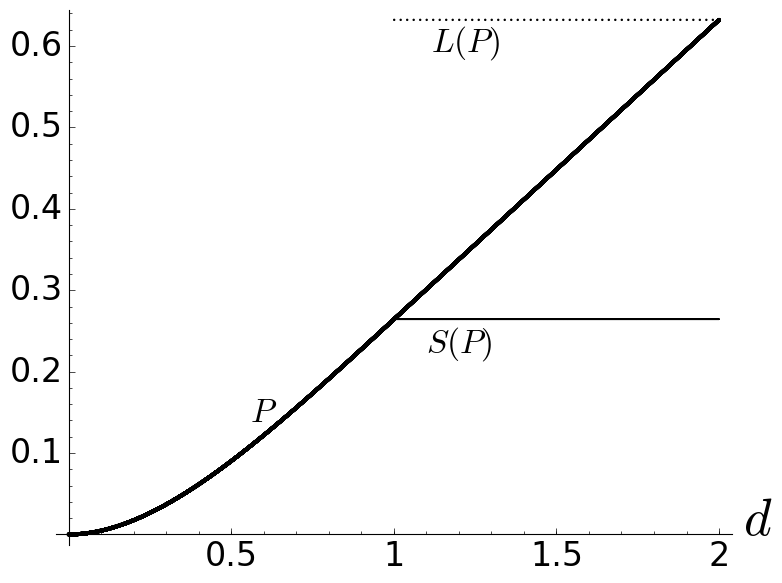
\includegraphics[scale=0.251]{cutvertices-planar.png}\hspace*{1cm}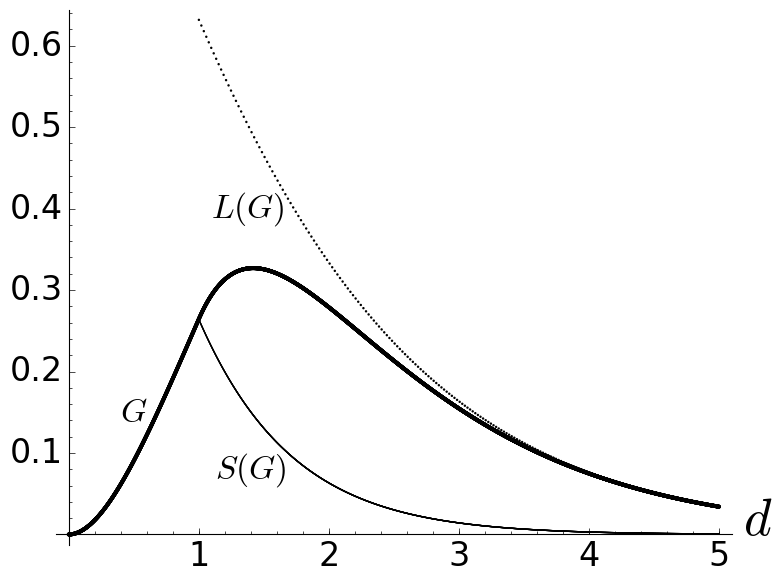
\includegraphics[scale=0.251]{cutvertices-ER.png}
\caption{Fraction of cut vertices in $P=P(n,m)$ and $G=G(n,m)$, where $m=m(n)$ is such that $2m/n\to d$.}
\label{fig:cv}
\end{figure}
\Cref{thm:planar_sub,thm:er_sub} show that $\cv{P}$ and $\cv{G}$ coincide asymptotically as long as $m\leq n/2+\bigo{n^{2/3}}$. However, \Cref{thm:planar_sup,thm:er_sup} reveal a completely different behaviour of $\cv{P}$ and $\cv{G}$ beyond this region (see also \Cref{fig:cv}). We could not find the results of \Cref{thm:er_sub,thm:er_sup} in literature and therefore, we provide sketches of their proofs in \Cref{sec:er}. In \Cref{sec:planar}, we show \Cref{thm:planar_sub,thm:planar_sup}. 
	
\section{Cut vertices in the \ER\ random graph}\label{sec:er}
To prove \Cref{thm:er_sub,thm:er_sup} on the number of cut vertices in the \ER\ random graph $G=G(n,m)$, we will use the following facts (see e.g. \cite{Bollobas2001}).
\begin{thm}\label{thm:er}
Let $k\in \N$, $G=G(n,m)$, $L=L(G)$ be the largest component of $G$, and $m=m(n)$ be such that $2m/n \to d\geq 0$. Then whp \textup{(i)} $v(L)=\left(\beta_d+\smallo{1}\right)n$, \textup{(ii)} the second largest component of $G$ has $\smallo{n}$ vertices, and \textup{(iii)} $\left|\left\{v\in V(G)\mid d_G(v)=k\right\}\right|=\left(e^{-d}d^k/k!+\smallo{1}\right) n$.
\end{thm}
{\itshape Sketch proofs of \Cref{thm:er_sub,thm:er_sup}.}~
We estimate the number $X^{(k)}$ of cut vertices in $G$ with $d_G(v)=k$ for $k\geq 2$. Let $X_v^{(k)}=1$ if $v\in V(G)$ is a cut vertex and $d_G(v)=k$, otherwise we set $X_v^{(k)}=0$. We construct $G$ conditioned on the event $d_G(v)=k$: We choose a random graph $G'$ on vertex set $[n]\setminus\{v\}$ with $m-k$ edges and then pick independently a set $N_v\subseteq [n]\setminus\{v\}$ for the $k$ neighbours of $v$. Now $v$ is not a cut vertex if and only if all $k$ vertices of $N_v$ lie in the same component of $G'$. As $G'$ is distributed like $G(n-1,m-k)$, \Cref{thm:er} implies that whp the largest component of $G'$ has $\left(\beta_d+\smallo{1}\right)n$ vertices, while all other components have $o(n)$ vertices. Together with \Cref{thm:er} this shows $\prob{X_v^{(k)}=1}=e^{-d}d^k/k! \cdot \left(1-\beta_d^k\right)+\smallo{1}$. Similarly, we obtain $\prob{X_v^{(k)}=X_w^{(k)}=1}=\left(e^{-d}d^k/k! \cdot \left(1-\beta_d^k\right)\right)^2+\smallo{1}$ for $v\neq w$. Hence, whp $X^{(k)}=\left(e^{-d}d^k(1-\beta_d^k)/k!+\smallo{1}\right)n$ by the first and second moment method. Due to \Cref{thm:er} there are $\smallo{n}$ vertices $v\in V(G)$ with $d_G(v)=\smallomega{1}$. Thus, whp $ \cv{G}=\left(\sum_{k\geq 2}X^{(k)}  + o(n)\right)/n=\sum_{k\geq 2}\left(e^{-d}d^k(1-\beta_d^k)/k!\right)+\smallo{1}=1-\left(d+e^{d\beta_d}-d\beta_d\right)e^{-d}+\smallo{1}$, which proves the statements on $\cv{G}$. Similarly, we show the assertions on $\cv{L}$ and $\cv{S}$. \qed

\section{Cut vertices in the random planar graph}\label{sec:planar}
\subsection[Average degree at most one]{Average degree at most one: Proof of \Cref{thm:planar_sub}}
\Cref{thm:planar_sub} is a direct consequence of the following well-known fact from \cite{Britikov1989}.
\begin{thm}[\hspace{1sp}\cite{Britikov1989}]\label{thm:non_complex}
Let $G=G(n,m)$ and $m=m(n)\leq n/2+\bigo{n^{2/3}}$. Then we have $\liminf_{n \to \infty}~ \prob{G \text{ has no components with at least two cycles}}>0$.	
\end{thm}
{\itshape Proof of \Cref{thm:planar_sub}.}~
Due to \Cref{thm:non_complex} we have  $\liminf_{n \to \infty}~ \prob{G \text{ is planar}}>0$. Therefore, each property that holds whp in $G(n,m)$ is also true whp in $P(n,m)$ as long as $m\leq n/2+\bigo{n^{2/3}}$. Hence, \Cref{thm:planar_sub} follows by \Cref{thm:er_sub}. \qed
	
\subsection{Graph decomposition and conditional random graphs}\label{sub:decomp}
To show \Cref{thm:planar_sup} we use the graph decomposition as in \cite{KangMosshammerSpruessel2020}. Given a graph $H$, the {\em complex part} $Q(H)$ of $H$ is the union of all components with at least two cycles. The remaining part $U(H):=H\setminus Q(H)$ is called the {\em non-complex part} and we define $n_U(H):=v(U(H))$ and $m_U(H):=e(U(H))$. The {\em core} $C(H)$ is the maximal subgraph of $Q(H)$ with minimum degree at least two. We note that $Q(H)$ arises from $C(H)$ by replacing each vertex by a rooted tree. The following results of Kang, Mo{\ss}hammer, and Spr\"{u}ssel \cite{KangMosshammerSpruessel2020} will be useful. 
	
\begin{thm}[\hspace{1sp}\cite{KangMosshammerSpruessel2020}]\label{thm:internal_structure}
Let $P=P(n,m)$, $Q=Q(P)$ the complex part of $P$, $C=C(P)$ the core, $L=L(P)$ the largest component, and $S=S(P)=P\setminus L$. Moreover, let $U=U(P)$ be the non-complex part of $P$, $n_U=v(U)$, and $m_U=e(U)$. Assume $m=m(n)$ is such that $n/2+\smallomega{n^{2/3}}\leq m \leq n+\smallo{n\left(\log n\right)^{-2/3}}$ and $2m/n \to d\in[1,2]$. Then whp \textup{(i)} $v(C)=\smallo{v(Q)}$, \textup{(ii)} $v(L)=\left(d-1+\smallo{1}\right)n$, \textup{(iii)} $n_U=\smallomega{1}$, \textup{(iv)} $m_U= n_U/2+\bigo{hn_U^{2/3}}$ for each function $h=h(n)=\smallomega{1}$, \textup{(v)} $\left|V(L)\triangle V(Q)\right|=\smallo{v(L)}$, and \textup{(vi)} $\left|V(S)\triangle V(U)\right|=\smallo{v(S)}$.
\end{thm}
\Cref{thm:internal_structure}(v) and (vi) imply that whp $\cv{L}=\cv{Q}+\smallo{1}$ and $\cv{S}=\cv{U}+\smallo{1}$. Furthermore, \Cref{thm:internal_structure}(ii) allows us to compute $\cv{P}$ once $\cv{L}$ and $\cv{S}$ are known. Thus, it suffices to determine $\cv{Q}$ and $\cv{U}$, which we will do in \Cref{sub:complex,sub:non_complex}, respectively. We will compute $\cv{Q}$ and $\cv{U}$ conditioned that $P$ satisfies some properties. Then we will use the following definition and lemma from \cite{KangMissethan2021} to deduce $\cv{Q}$ and $\cv{U}$.
	
\begin{definition}[{\hspace{1sp}\cite[Definition 3.1]{KangMissethan2021}}]\label{def:feasible} 
Given a class $\mathcal{A}$ of graphs let $\mathcal{A}(n)$ be the subclass containing those graphs with vertex set $[n]$.
Let $S$ be a set  and $\Phi:\mathcal{A}\to S$ a function. We say that a sequence $\mathbf{a}=(a_n)_{n\in \N}$ is {\em feasible} for $\left(\mathcal{A}, \Phi\right)$ if for each $n \in \N$  there is a graph $H \in \mathcal{A}(n)$ such that $\Phi(H)=a_n$. Furthermore, for each $n\in \N$ we write $\left(A\mid\mathbf{a}\right)(n)$ for a graph chosen uniformly at random from the set $\left\{H \in \mathcal{A}(n): \Phi(H)=a_n\right\}$. We will often omit the dependence on $n$ and write $A\mid\mathbf{a}$ instead of $\left(A\mid\mathbf{a}\right)(n)$.
\end{definition}
\begin{lem}[{\hspace{1sp}\cite[Lemma 3.2]{KangMissethan2021}}]\label{lem:conditional_random_graphs}
Let $\mathcal{A}$ be a class of graphs, $A=A(n)$ a graph chosen uniformly at random from $\mathcal{A}(n)$, $S$ a set, $\Phi:\mathcal{A}\to S$ a function, and $\mathcal{R}$ a graph property, i.e. $\mathcal{R}$ is a set of graphs. If for every sequence $\mathbf{a}=(a_n)_{n\in \N}$ that is feasible for $\left(\mathcal{A}, \Phi\right)$ whp $A\mid\mathbf{a}\in \mathcal{R}$, then we have whp $A \in \mathcal{R}$.
\end{lem}
	
\subsection{Cut vertices in the complex part}\label{sub:complex}
Using the concept of \lq conditional\rq\ random graphs (see \Cref{def:feasible} and \Cref{lem:conditional_random_graphs}) we will determine $\cv{Q(P)}$ in this section. For a given core $C$ and $q\in\N$ we denote by $Q(C,q)$ a graph chosen uniformly at random from the class of all complex parts which have $C$ as its core and vertex set $[q]$. We observe that $Q(C,q)$ is distributed like $Q(P)$ conditioned on the event $C(P)=C$ and $v(Q(P))=q$. Furthermore, $Q(C,q)$ can be constructed by choosing a random forest $F$ on vertex set $[q]$ with $v(C)$ many tree components such that the vertices from $C$ lie all in different tree components. Then we obtain $Q(C,q)$ by replacing each vertex $v$ in $C$ by the tree component of $F$ which is rooted at $v$. Therefore, we estimate first $\cv{F}$ in \Cref{lem:cut_vertices_forest} and then deduce $\cv{Q(C,q)}$ in \Cref{lem:cut_vertices_complex}. To that end, we denote by $F(n,t)$ a forest chosen uniformly at random from the class of all forests on vertex set $[n]$ having exactly $t$ trees as components such that the vertices $1, \ldots, t$ lie all in different tree components.
\begin{lem}\label{lem:cut_vertices_forest}
Let $t=t(n)=\smallo{n}$ and $F=F(n,t)$ be the random forest. Then we have whp $\cv{F}=1-e^{-1}+\smallo{1}$.
\end{lem}
\begin{proof}
A vertex $v\in[n]\setminus[t]$ is a cut vertex in $F$ if and only if $d_F(v)\neq 1$. We set $X_v=1$ if $d_F(v)= 1$ and $X_v=0$ otherwise. As $t=\smallo{n}$, it suffices to prove whp $\sum_{v\in[n]\setminus[t]}X_v=\left(e^{-1}+\smallo{1}\right)n$. Each realisation $H$ of $F$ with $d_H(v)=1$ can be constructed by first choosing a forest $H'$ on vertex set $[n]\setminus\left\{v\right\}$ with $t$ tree components such that the vertices in $[t]$ lie all in different tree components. Then we obtain $H$ by picking a vertex $v'\in [n]\setminus\left\{v\right\}$ and adding the edge $vv'$ in $H'$. This implies $\prob{X_v=1}=t(n-1)^{n-t-2}\cdot(n-1)/\left(tn^{n-t-1}\right)=e^{-1}+\smallo{1}$. Similarly, we obtain $\prob{X_v=X_w=1}=t(n-2)^{n-t-3}\cdot(n-2)^2/\left(tn^{n-t-1}\right)=e^{-2}+\smallo{1}$ for all $v\neq w$. The statement follows by the first and second moment method.
\end{proof}
	
\begin{lem}\label{lem:cut_vertices_complex}
For each $n\in\N$, let $C=C(n)$ be a core, $q=q(n)\in\N$, and $Q=Q(C,q)$ be the random complex part with core $C$ and vertex set $[q]$. If $v(C)=\smallo{q}$, then whp $\cv{Q}=1-e^{-1}+\smallo{1}$.
\end{lem}
\begin{proof}
W.l.o.g. we assume $V(C)=[v(C)]$. We construct $Q$ by picking a random forest $F=F(q,v(C))$ and replacing each vertex $v$ in $C$ by the tree component of $F$ which is rooted at $v$. A vertex $v\in [q]\setminus[v(C)]$ is a cut vertex in $Q$ if and only if it is a cut vertex in $F$. Together with the fact $v(C)=\smallo{q}$ it implies  whp $\cv{Q}=\cv{F}+\smallo{1}$. Hence, whp $\cv{Q}=1-e^{-1}+\smallo{1}$ by \Cref{lem:cut_vertices_forest}.
\end{proof}
	
Finally, we use \Cref{lem:conditional_random_graphs} to transfer the result on the fraction of cut vertices in $Q(C,q)$ from \Cref{lem:cut_vertices_complex} to the complex part $Q(P)$ of $P$.
\begin{lem}\label{lem:cv_complex}
Let $P=P(n,m)$ and $Q=Q(P)$ be the complex part of $P$. Assume $m=m(n)$ is such that $n/2+\smallomega{n^{2/3}}\leq m \leq n+\smallo{n\left(\log n\right)^{-2/3}}$ and $2m/n \to d\in[1,2]$. Then whp $\cv{Q}=1-e^{-1}+\smallo{1}$.
\end{lem}
\begin{proof}
To use \Cref{lem:conditional_random_graphs}, let $\mathcal{A}(n)$ be the class of planar graphs $H$ with vertex set $[n]$ and $m$ edges satisfying $v(C(H))=\smallo{v(Q(H))}$. By \Cref{thm:internal_structure}(i) we have whp $P\in\mathcal{A}:=\cup_{n\in\N}\mathcal{A}(n)$. Let $\Phi$ be such that $\Phi(H)=\left(C(H), v(Q(H))\right)$ for each $H\in\mathcal{A}$, $A=A(n)$ be a graph chosen uniformly at random from $\mathcal{A}(n)$, and $\mathbf{a}=(C_n, q_n)_{n\in\N}$ be a sequence that is feasible for $\left(\mathcal{A},\Phi\right)$. We note that $Q(A \mid \mathbf{a})$ is distributed like the random complex part $Q(C_n, q_n)$. Thus, we get by \Cref{lem:cut_vertices_complex} that whp $\cv{Q(A \mid \mathbf{a})}=1-e^{-1}+\smallo{1}$. Combining it with \Cref{lem:conditional_random_graphs} yields whp $\cv{Q(A)}=1-e^{-1}+\smallo{1}$. This shows the statement, since whp $P\in\mathcal{A}$.
\end{proof}
	
\subsection{Cut vertices in the non-complex part}\label{sub:non_complex}
 For given $n,m\in\N$ let $U(n,m)$ be a graph chosen uniformly at random from all graphs with vertex set $[n]$ and $m$ edges in which every component has at most one cycle. First we will determine $\cv{U(n,m)}$ and then deduce $\cv{U(P)}$.
\begin{lem}\label{lem:cv_non_complex}
Let $U=U(n,m)$ and $m=m(n)\leq n/2+\bigo{n^{2/3}}$ such that $2m/n \to d\in[0,1]$. Then whp $\cv{U}=1-(d+1)e^{-d}+\smallo{1}$.	
\end{lem}
\begin{proof}
The assertion follows by combining \Cref{thm:er_sub,thm:non_complex}. 
\end{proof}
\begin{lem}\label{lem:cv_non_complex1}
Let $P=P(n,m)$ and $U=U(P)$ be the non-complex part of $P$. Assume $m=m(n)$ is such that $n/2+\smallomega{n^{2/3}}\leq m \leq n+\smallo{n\left(\log n\right)^{-2/3}}$ and $2m/n \to d\in[1,2]$. Then whp $\cv{U}=1-2e^{-1}+\smallo{1}$.
\end{lem}
\begin{proof}
To use \Cref{lem:conditional_random_graphs}, let $\mathcal{A}(n)$ be the class of planar graphs $H$ with vertex set $[n]$ and $m$ edges satisfying $n_U(H)=\smallomega{1}$ and $m_U(H)=n_U(H)/2+\bigo{n_U(H)^{2/3}}$. By \Cref{thm:internal_structure}(iii) and (iv) we can choose the implicit constants in these equations such that $P\in\mathcal{A}:=\cup_{n\in\N}\mathcal{A}(n)$ with a probability of at least $1-\delta$, where $\delta>0$ is a given constant. Let $\Phi$ be such that $\Phi(H)=\left(n_U(H), m_U(H)\right)$ for each $H\in\mathcal{A}$, $A=A(n)$ be a graph chosen uniformly at random from $\mathcal{A}(n)$ and $\mathbf{a}=(\nu_n, \mu_n)_{n\in\N}$ be a sequence that is feasible for $\left(\mathcal{A},\Phi\right)$. By \Cref{lem:cv_non_complex} we get whp $\cv{U(A \mid \mathbf{a})}=1-2e^{-1}+\smallo{1}$, as $U(A \mid \mathbf{a})$ is distributed like $U(\nu_n, \mu_n)$. Together with \Cref{lem:conditional_random_graphs} this implies whp $\cv{U(A)}=1-2e^{-1}+\smallo{1}$. Using $\prob{P\in\mathcal{A}}>1-\delta$, we obtain that $\cv{U(P)}=1-2e^{-1}+\smallo{1}$ holds with a probability of at least $1-2\delta$. The statement follows, as $\delta>0$ was arbitrary.
\end{proof}
	
\subsection[Average degree between one and two]{Average degree between one and two: Proof of \Cref{thm:planar_sup}}
Let $Q=Q(P)$ be the complex part of $P$. By \Cref{thm:internal_structure}(v) we have whp $\cv{L}=\cv{Q}+\smallo{1}$ and \Cref{lem:cv_complex} states that whp $\cv{Q}=1-e^{-1}+\smallo{1}$. Thus, whp $\cv{L}=1-e^{-1}+\smallo{1}$. Due to \Cref{thm:internal_structure}(vi) and \Cref{lem:cv_non_complex1} we have whp $\cv{S}=\cv{U}+\smallo{1}=1-2e^{-1}+\smallo{1}$, where $U=U(P)$ is the non-complex part of $P$. Finally, by \Cref{thm:internal_structure}(ii) we have whp $v(L)=\left(d-1+\smallo{1}\right)n$. Thus, we get whp $\cv{P}=\left(\cv{L}v(L)+\cv{S}v(S)\right)/n=1-(3-d)e^{-1}+\smallo{1}$. \qed